\documentclass[aspectratio=169]{beamer}

\usetheme{Boadilla}
\usefonttheme{professionalfonts}
\setbeamertemplate{navigation symbols}{}
\setbeamertemplate{itemize items}[circle]
\setbeamertemplate{enumerate items}[default]
\setbeamertemplate{headline}{}

\usepackage[utf8]{inputenc}
\usepackage[T1]{fontenc}
\usepackage{lmodern}
\usepackage{amsmath}
\usepackage{booktabs}
\usepackage{tabularx}
\usepackage{array}
\usepackage{hyperref}
\usepackage[strings]{underscore}
\usepackage{listings}
\usepackage{tikz}
\usetikzlibrary{arrows.meta,positioning,fit,calc,shapes.geometric}
\usepackage{xcolor}

\definecolor{courseblue}{HTML}{12355B}
\definecolor{coursegold}{HTML}{C98A2E}
\definecolor{courseice}{HTML}{EEF3F8}
\definecolor{coursegreen}{HTML}{2F6B4F}
\definecolor{coursegray}{HTML}{4B5563}
\definecolor{codebg}{HTML}{F7F9FC}
\definecolor{codecomment}{HTML}{5E6C84}
\definecolor{codestring}{HTML}{0B6E4F}

\setbeamercolor{palette primary}{bg=courseblue,fg=white}
\setbeamercolor{palette secondary}{bg=coursegold,fg=white}
\setbeamercolor{palette tertiary}{bg=courseblue,fg=white}
\setbeamercolor{palette quaternary}{bg=coursegold,fg=white}
\setbeamercolor{structure}{fg=courseblue}
\setbeamercolor{frametitle}{bg=courseice,fg=courseblue}
\setbeamercolor{title}{fg=courseblue}
\setbeamercolor{block title}{bg=courseblue,fg=white}
\setbeamercolor{block body}{bg=courseice,fg=black}
\setbeamercolor{normal text}{fg=black,bg=white}
\setbeamercolor{alerted text}{fg=coursegold}

\setbeamerfont{footline}{size=\scriptsize}

\setbeamertemplate{footline}{
  \leavevmode
  \hbox{
    \begin{beamercolorbox}[wd=.33\paperwidth,ht=2.8ex,dp=1.2ex,leftskip=0.8em]{palette primary}%
      University of Trieste
    \end{beamercolorbox}%
    \begin{beamercolorbox}[wd=.49\paperwidth,ht=2.8ex,dp=1.2ex,center]{palette tertiary}%
      \coursename{} \textbar{} \coursecode
    \end{beamercolorbox}%
    \begin{beamercolorbox}[wd=.18\paperwidth,ht=2.8ex,dp=1.2ex,right,rightskip=0.8em]{palette secondary}%
      \insertframenumber{} / \inserttotalframenumber
    \end{beamercolorbox}%
  }
}

\hypersetup{
  colorlinks=true,
  linkcolor=courseblue,
  urlcolor=coursegreen
}

\lstdefinestyle{coursepython}{
  language=Python,
  basicstyle=\ttfamily\footnotesize,
  keywordstyle=\color{courseblue}\bfseries,
  commentstyle=\color{codecomment}\itshape,
  stringstyle=\color{codestring},
  showstringspaces=false,
  columns=fullflexible,
  keepspaces=true,
  frame=single,
  framerule=0.6pt,
  rulecolor=\color{courseblue},
  backgroundcolor=\color{codebg},
  xleftmargin=0.4em,
  xrightmargin=0.4em,
  aboveskip=0.4em,
  belowskip=0.2em
}

\newcommand{\coursename}{Data-driven Systems Engineering}
\newcommand{\coursecode}{440MI / 305SM}
\newcommand{\coursefooter}{}

\newcommand{\learninggoals}[1]{
  \begin{block}{Learning goals}
  #1
  \end{block}
}

\newcommand{\repoactivity}[1]{
  \begin{block}{Repo activity}
  #1
  \end{block}
}

\newcommand{\readinglist}[1]{
  \begin{block}{Papers and materials}
  {\footnotesize #1}
  \end{block}
}

\newcommand{\coursecontextframe}[5]{
  \begin{frame}{Course Map and Running Cases}
  \centering
  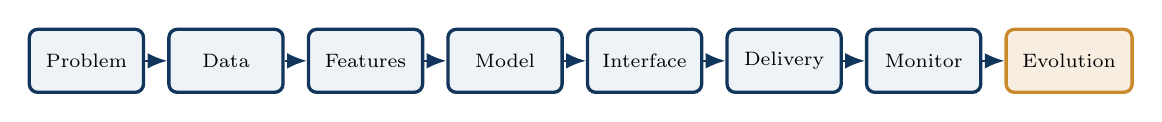
\begin{tikzpicture}[node distance=0.28cm]
  \node[flowbox, minimum width=1.45cm, minimum height=0.8cm] (problem) {\scriptsize Problem};
  \node[flowbox, minimum width=1.45cm, minimum height=0.8cm, right=of problem] (data) {\scriptsize Data};
  \node[flowbox, minimum width=1.45cm, minimum height=0.8cm, right=of data] (features) {\scriptsize Features};
  \node[flowbox, minimum width=1.45cm, minimum height=0.8cm, right=of features] (model) {\scriptsize Model};
  \node[flowbox, minimum width=1.45cm, minimum height=0.8cm, right=of model] (interface) {\scriptsize Interface};
  \node[flowbox, minimum width=1.45cm, minimum height=0.8cm, right=of interface] (delivery) {\scriptsize Delivery};
  \node[flowbox, minimum width=1.45cm, minimum height=0.8cm, right=of delivery] (monitor) {\scriptsize Monitor};
  \node[accentbox, minimum width=1.6cm, minimum height=0.8cm, right=of monitor] (evolution) {\scriptsize Evolution};
  \foreach \a/\b in {problem/data,data/features,features/model,model/interface,interface/delivery,delivery/monitor,monitor/evolution} {
    \draw[arrow] (\a) -- (\b);
  }
  \end{tikzpicture}

  \vspace{0.5em}
  \begin{block}{Today in the course}
  \textbf{Focus:} #1

  \textbf{Bridge:} #2
  \end{block}

  \begin{columns}[T]
  \column{0.48\textwidth}
  \begin{block}{Fraud case}
  {\footnotesize #3}
  \end{block}
  \column{0.48\textwidth}
  \begin{block}{Pasteurization case}
  {\footnotesize #4}
  \end{block}
  \end{columns}

  \vspace{0.3em}
  {\footnotesize \textbf{Course thread:} #5}
  \coursefooter
  \end{frame}
}

\newcommand{\classclosingframe}[4]{
  \begin{frame}{From This Class to the Next}
  \begin{block}{What stays with us}
  #1
  \end{block}

  \begin{columns}[T]
  \column{0.48\textwidth}
  \begin{block}{Project use}
  {\footnotesize #2}
  \end{block}
  \column{0.48\textwidth}
  \begin{block}{Next connection}
  {\footnotesize #3}
  \end{block}
  \end{columns}

  \vspace{0.3em}
  {\footnotesize \textbf{Course thread:} #4}
  \coursefooter
  \end{frame}
}

\tikzset{
  flowbox/.style={
    rounded corners=3pt,
    draw=courseblue,
    fill=courseice,
    very thick,
    minimum width=2.2cm,
    minimum height=0.9cm,
    align=center,
    font=\small
  },
  accentbox/.style={
    rounded corners=3pt,
    draw=coursegold,
    fill=coursegold!15,
    very thick,
    minimum width=2.2cm,
    minimum height=0.9cm,
    align=center,
    font=\small
  },
  arrow/.style={
    -{Latex[length=2.5mm,width=2mm]},
    thick,
    draw=courseblue
  }
}


\title{Class 15: Encoding and Embedding Practice}
\subtitle{Represent the categories, inspect the result, and state what the evidence supports}
\author{\coursename}
\date{23 October}

\begin{document}

\frame{\titlepage \coursefooter}

\begin{frame}{Attributes in the prepared Titanic dataset}
\footnotesize
\begin{tabularx}{\textwidth}{>{\ttfamily}l X l}
\toprule
Attribute & Description & Role in this activity \\
\midrule
sex & Passenger sex recorded in the dataset & Nominal feature \\
pclass & Ticket class: 1st, 2nd, or 3rd & Ordered feature \\
embarked & Port of embarkation: C = Cherbourg, Q = Queenstown, S = Southampton & Nominal feature \\
age & Passenger age in years; missing values already imputed & Numeric feature \\
fare & Passenger fare & Numeric feature \\
sibsp & Number of siblings and spouses aboard & Numeric feature \\
parch & Number of parents and children aboard & Numeric feature \\
survived & Outcome: 0 = did not survive; 1 = survived & Target \\
partition & Marks each row as train or test & Split marker; not a feature \\
\bottomrule
\end{tabularx}

\vspace{0.5em}
\begin{alertblock}{Scope of the supplied CSV}
This prepared file contains eight passenger attributes plus the train/test marker. It is a selected, imputed subset for the activity; other fields from the full Titanic dataset are not included.
\end{alertblock}
\coursefooter
\end{frame}

\begin{frame}{Today's question: is this a useful representation?}
\begin{itemize}
\item Build encodings for Titanic categories and inspect the resulting feature matrix.
\item Explore how the categories relate to survival, without fitting a predictive model.
\item Construct a PCA projection of passenger profiles grouped by embarkation port.
\item Separate evidence about representation quality from evidence about model contribution.
\end{itemize}
\begin{block}{Prepared data}
Use a prepared Titanic train/test split with missing feature values already handled for this exercise. Imputation choices are the focus of Class 16; the solution notebook shows the split-safe preparation used to create the fixture.
\end{block}
\vspace{0.2em}
\centering\small\href{../notebooks/Class15_Titanic_Imputed.csv}{Download the prepared Titanic train/test fixture (CSV)}
\coursefooter
\end{frame}

\begin{frame}{Pick a representation that matches the category}
\begin{tabularx}{\textwidth}{>{\ttfamily}l l X}
\toprule
Feature & Structure & Representation to inspect \\
\midrule
\texttt{sex} & Nominal, two categories & One-hot; no natural order \\
\texttt{embarked} & Nominal, three ports & One-hot; check unseen-category behavior \\
\texttt{pclass} & Ordered categories & Compare one-hot with ordinal codes $1,2,3$ \\
\bottomrule
\end{tabularx}
\vspace{0.7em}
\begin{itemize}
\item Ordinal codes preserve order but add a distance assumption: the step from 1 to 2 equals the step from 2 to 3.
\item One-hot encoding preserves category identity without adding an order.
\item A learned or PCA-based embedding assigns coordinates; what those coordinates mean depends on how they were learned.
\end{itemize}
\coursefooter
\end{frame}

\begin{frame}{One-hot turns categories into explicit columns}
\small
\centering
\begin{tabular}{c c c | c c | c c c}
\toprule
 & \multicolumn{2}{c|}{Input categories} & \multicolumn{2}{c|}{Output: sex} & \multicolumn{3}{c}{Output: embarked} \\
Passenger & \texttt{sex} & \texttt{port} & female & male & C & Q & S \\
\midrule
A & female & C & \colorbox{coursegold}{\textcolor{white}{\makebox[1.5em]{\textbf{1}}}} & \colorbox{courseice}{\makebox[1.5em]{0}} & \colorbox{coursegold}{\textcolor{white}{\makebox[1.5em]{\textbf{1}}}} & \colorbox{courseice}{\makebox[1.5em]{0}} & \colorbox{courseice}{\makebox[1.5em]{0}} \\
B & male & S & \colorbox{courseice}{\makebox[1.5em]{0}} & \colorbox{coursegold}{\textcolor{white}{\makebox[1.5em]{\textbf{1}}}} & \colorbox{courseice}{\makebox[1.5em]{0}} & \colorbox{courseice}{\makebox[1.5em]{0}} & \colorbox{coursegold}{\textcolor{white}{\makebox[1.5em]{\textbf{1}}}} \\
C & female & Q & \colorbox{coursegold}{\textcolor{white}{\makebox[1.5em]{\textbf{1}}}} & \colorbox{courseice}{\makebox[1.5em]{0}} & \colorbox{courseice}{\makebox[1.5em]{0}} & \colorbox{coursegold}{\textcolor{white}{\makebox[1.5em]{\textbf{1}}}} & \colorbox{courseice}{\makebox[1.5em]{0}} \\
\bottomrule
\end{tabular}

\vspace{0.9em}
\begin{columns}[T]
\column{0.48\textwidth}
\begin{block}{What changed?}
One category becomes one column. The active column records the observed category; no artificial order is introduced.
\end{block}
\column{0.48\textwidth}
\begin{alertblock}{What to check?}
Fit columns on training data. Confirm expected levels and document how an unseen value is handled at transform time.
\end{alertblock}
\end{columns}
\coursefooter
\end{frame}

\begin{frame}{First evaluate representation quality}
\small
\begin{tabularx}{\textwidth}{>{\bfseries}l X X}
\toprule
Check & Evidence to collect & What it tells us \\
\midrule
Validity & Learned categories and output names & Expected levels are preserved \\
Robustness & Transform a row with an unseen value & Behavior is documented \\
Complexity & Output columns and matrix density & Size and sparsity are manageable \\
Exploratory signal & Category counts and target rates & Group differences suggest a hypothesis \\
\bottomrule
\end{tabularx}
\vspace{0.3em}
\begin{alertblock}{Scope of this evidence}
These checks assess the representation and describe the data; they do not establish predictive improvement.
\end{alertblock}
\coursefooter
\end{frame}

\begin{frame}{Check category coverage and compare group rates}
\begin{columns}[T]
\column{0.72\textwidth}
\centering
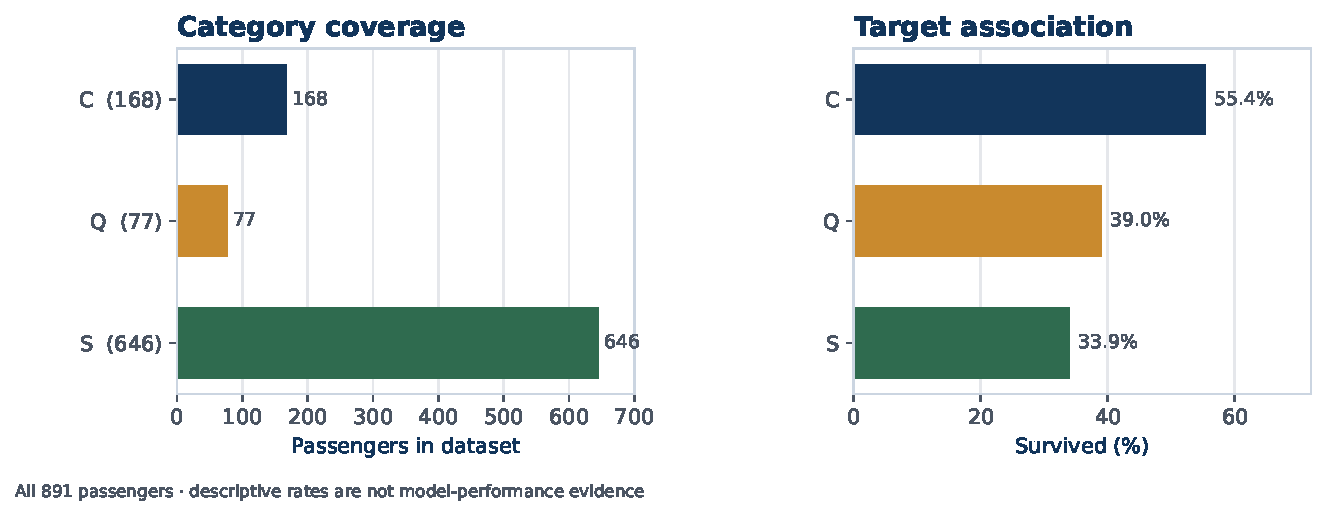
\includegraphics[width=\linewidth]{figures/class15_embarked_diagnostics.pdf}
\column{0.26\textwidth}
\small
\begin{block}{Read the chart}
All ports appear in train, but their counts differ. Compare the survival rates while keeping those sample sizes in view.
\end{block}
\end{columns}
\vspace{0.3em}
\begin{alertblock}{Interpretation}
These are descriptive differences in this sample. They do not show that encoding improves held-out predictions.
\end{alertblock}
\coursefooter
\end{frame}

\begin{frame}{Association heatmaps: read each statistic on its own scale}
\centering
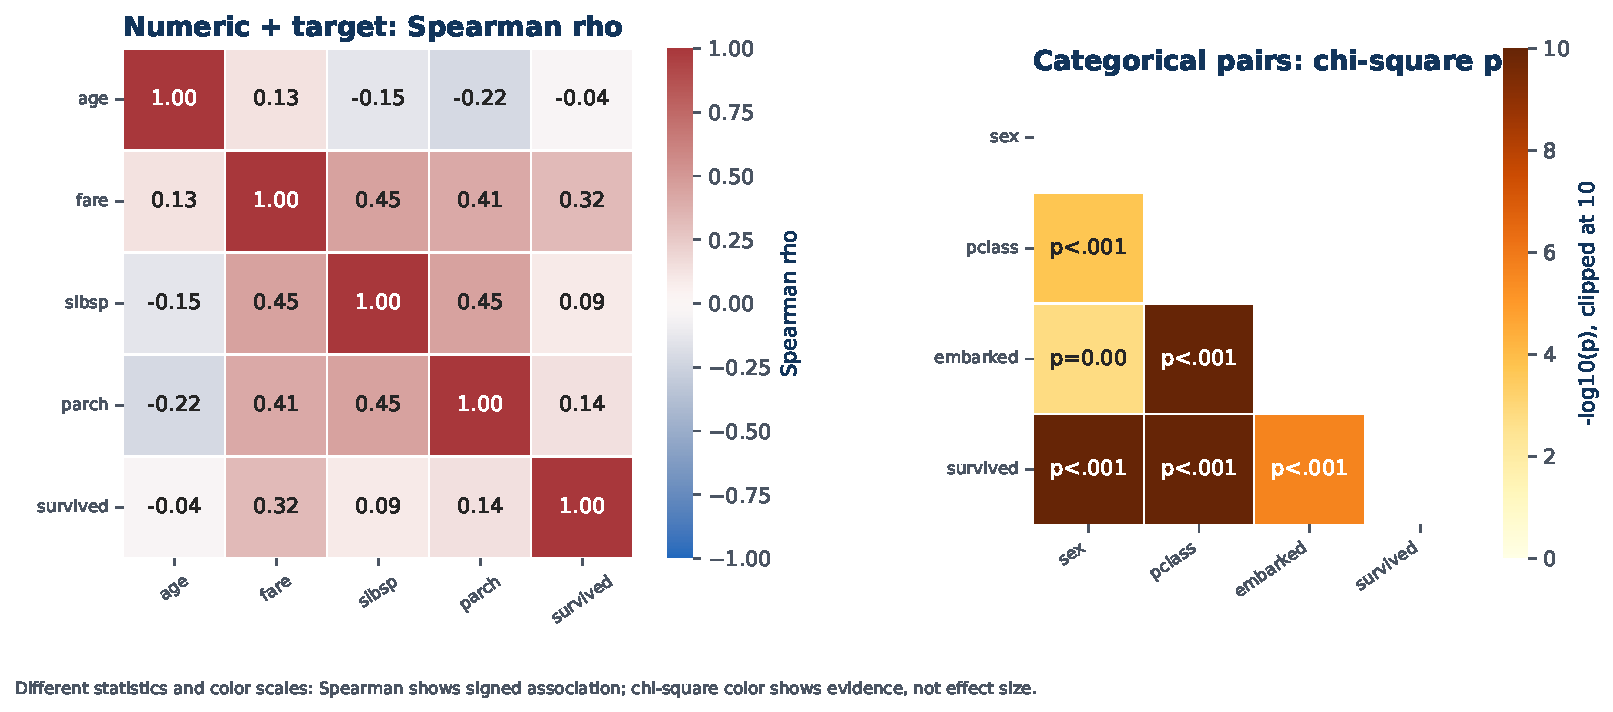
\includegraphics[width=0.91\textwidth,height=0.52\textheight,keepaspectratio]{figures/class15_association_heatmaps.pdf}
\vspace{0.2em}
\begin{alertblock}{Interpretation}
Spearman $\rho$ shows signed rank association. Chi-squared colors show evidence against independence via $p$-values, not effect size. The panels are not directly comparable.
\end{alertblock}
\coursefooter
\end{frame}

\begin{frame}{PCA shows how original features align with the profile axes}
\begin{columns}[T]
\column{0.64\textwidth}
\centering
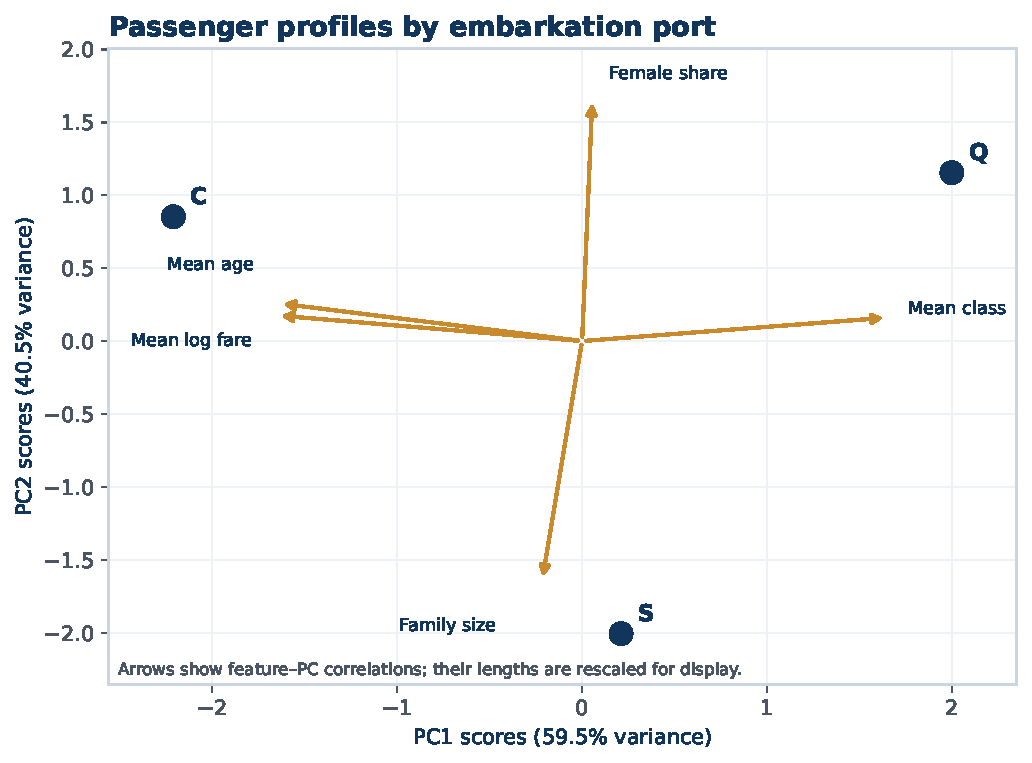
\includegraphics[width=\linewidth,height=0.70\textheight,keepaspectratio]{figures/class15_port_profile_pca.pdf}
\column{0.32\textwidth}
\footnotesize
\begin{itemize}
\item Points: three port profiles, built without \texttt{survived}.
\item Arrows: correlations of original features with PC1 and PC2.
\item Similar directions suggest features that vary together in these profiles.
\end{itemize}
\begin{alertblock}{Scope}
Two PCs explain 100\% here because there are only three centered profiles. This is exploratory, not evidence of predictive value.
\end{alertblock}
\end{columns}
\coursefooter
\end{frame}

\begin{frame}{One-hot PCA is not a useful port embedding here}
\begin{itemize}
\item Three one-hot port columns have at most two independent directions after centering.
\item PCA to two components therefore keeps all centered variation; it mostly rotates the same information.
\item The resulting coordinates do not learn that two ports are behaviorally or predictively similar.
\item Use the profile PCA as a small visualization exercise; keep one-hot as the clear baseline representation.
\end{itemize}
\begin{block}{Representation quality today}
Check that categories are preserved, the matrix is manageable, unknown values are handled, and any visual or target association is interpreted within its limits.
\end{block}
\coursefooter
\end{frame}

\begin{frame}{Can we say encoding contributed to modeling? Not yet.}
\begin{columns}[T]
\column{0.48\textwidth}
\textbf{We can assess today}
\begin{itemize}
\item Correctness and category coverage
\item Unknown-category handling
\item Number and density of features
\item Descriptive association with the target
\item Structure of the PCA profile plot
\end{itemize}
\column{0.48\textwidth}
\textbf{We cannot claim today}
\begin{itemize}
\item Better generalization
\item Higher predictive performance
\item That an embedding beats one-hot
\item That target association adds value alongside other features
\end{itemize}
\end{columns}
\vspace{0.5em}
\begin{alertblock}{Conclusion}
Encoding changes how a model receives information; it does not create new information by itself. Measuring predictive contribution requires a downstream model.
\end{alertblock}
\coursefooter
\end{frame}

\begin{frame}{How Class 18 will test contribution fairly}
\begin{enumerate}
\item Keep the same train/test split and the same downstream estimator.
\item Compare a baseline without the feature, one-hot \texttt{embarked}, and any candidate embedding.
\item Fit every learned transformation on training data only; evaluate once on the held-out test data.
\item Choose a suitable metric in advance (e.g., ROC AUC or balanced accuracy) and compare the change, not just one score.
\item Repeat across folds or seeds if time permits; report uncertainty and added complexity.
\end{enumerate}
\begin{block}{Today's deliverable}
A representation table, a short association interpretation, the PCA profile plot, and one explicit claim the evidence does \emph{not} support yet.
\end{block}
\coursefooter
\end{frame}

\begin{frame}{Debrief and transition}
\begin{itemize}
\item Which encoding assumptions were reasonable for \texttt{sex}, \texttt{embarked}, and \texttt{pclass}?
\item Did the PCA plot describe category profiles, or did it prove predictive usefulness?
\item Which representation would you carry forward as a baseline, and why?
\end{itemize}
\begin{block}{Next: Class 16}
Feature engineering returns to the raw data and examines cleaning, curation, missing values, construction, and selection. The prepared table today keeps that imputation discussion in its proper session.
\end{block}
\coursefooter
\end{frame}

\end{document}
